\section{Problem 1}
\subsection{Technics}

    \begin{frame}
        \frametitle{Problem 1 - Calculating Jordan Canonical Form}
        Using Eigen Library(C++):
        \begin{itemize}
            \item Compute eigenvalues using EigenSolver.
            \item Compute vector \(d_i\) and \(j_i\) associated with each eigenvalue \(\lambda_i\).
            \item Construct the Jordan block for Jordan Canonical Form.
        \end{itemize}
    \end{frame}

    \begin{frame}[fragile]
        \frametitle{Problem 1 - Details of Our Codes}
        \begin{itemize}
            \item Cauculate every eigenvalue of \(M\) and store them in vector \(eigenvalue\), remove the repeat eigenvalues.
        \end{itemize}
        \begin{codeblock}{c++}{C++ Codes}
    std::vector<double> eigenvalue;
    Eigen::EigenSolver<Eigen::MatrixXd> es(mat_in);
    eigenvalue.push_back(es.eigenvalues()[0].real());
    for (int eig = 1; eig < es.eigenvalues().size(); eig++){
        if(abs(es.eigenvalues()[eig].real() - eigenvalue[eigenvalue.size() - 1]) > 0.01){
            eigenvalue.push_back(es.eigenvalues()[eig].real()); }
        else{}
    }
        \end{codeblock}
    \end{frame}

    \begin{frame}[fragile]
        \frametitle{Problem 1 - Details of Our Codes}
        \begin{itemize}
            \item Cauculate \(dim(ker(M_\lambda^k))\), stop adding \(k\) until \(rank(M_\lambda^k)\) stop changing.
        \end{itemize}
        \begin{codeblock}{c++}{C++ Codes}
    Eigen::FullPivLU<Eigen::MatrixXd> lu_decomp(mat_lambda_power);
    int dimker = dim - lu_decomp.rank();
    if(DimKer.size() == 0){
        DimKer.push_back(dimker);
        last_dimker = dimker;}
    else{
        if(last_dimker != dimker){
            DimKer.push_back(dimker);
            last_dimker = dimker;}
        else{con_pow = 0;}}    
        \end{codeblock}
    \end{frame}

    \begin{frame}[fragile]
        \frametitle{Problem 1 - Details of Our Codes}
        \begin{itemize}
            \item Cauculate \(d_i\) according to \(dim(ker(M_\lambda^k))\).
            \item Cauculate \(j_i\) according to \(d_i\).
        \end{itemize}
        \begin{codeblock}{c++}{C++ Codes}
    for (int m = 0; m < DimKer.size(); m++) {
        if (m == 0) { d.push_back(DimKer[m]); }
        else { d.push_back(DimKer[m] - DimKer[m - 1]);}}
    D.push_back(d); 
    for (int n = 0; n < DimKer.size(); n++) {
        if (n == 0) { j.push_back(d[DimKer.size() - 1]); }
        else { j.push_back(d[DimKer.size() - n - 1] - d[DimKer.size() - n]); }}
    J.push_back(j);
        \end{codeblock}
    \end{frame}

    \begin{frame}[fragile]
        \frametitle{Problem 1 - Details of Our Codes}
        \begin{itemize}
            \item Show Jordan Canonical Form according to each \(\lambda_i\) and its associated \(d_i,j_i\).
        \end{itemize}
        \begin{codeblock}{c++}{C++ Codes}
for (int itr = 0; itr < eigenvalue.size(); itr++){
    for (int sub_j=0; sub_j<J[itr].size();sub_j++){
        for (int num_sub_j=0;num_sub_j<J[itr][sub_j];num_sub_j++){
            int end_row = start_row + J[itr].size() - sub_j;
            for (int sub_row=start_row;sub_row<end_row;sub_row++){
                for (int sub_col=start_row;sub_col<end_row;sub_col++){
                    if(sub_row==sub_col){mat_Jordan(sub_row,sub_col) = eigenvalue[itr];}
                    else if(sub_col == sub_row+1){mat_Jordan(sub_row,sub_col) = 1;}}} 
                start_row = end_row;}}}
        \end{codeblock}
    \end{frame}

    \subsection{Results}
    \begin{frame}
        \frametitle{Problem 1 - Program Result}
        % \framesubtitle{子标题}
        
        \begin{figure}
            \centering
            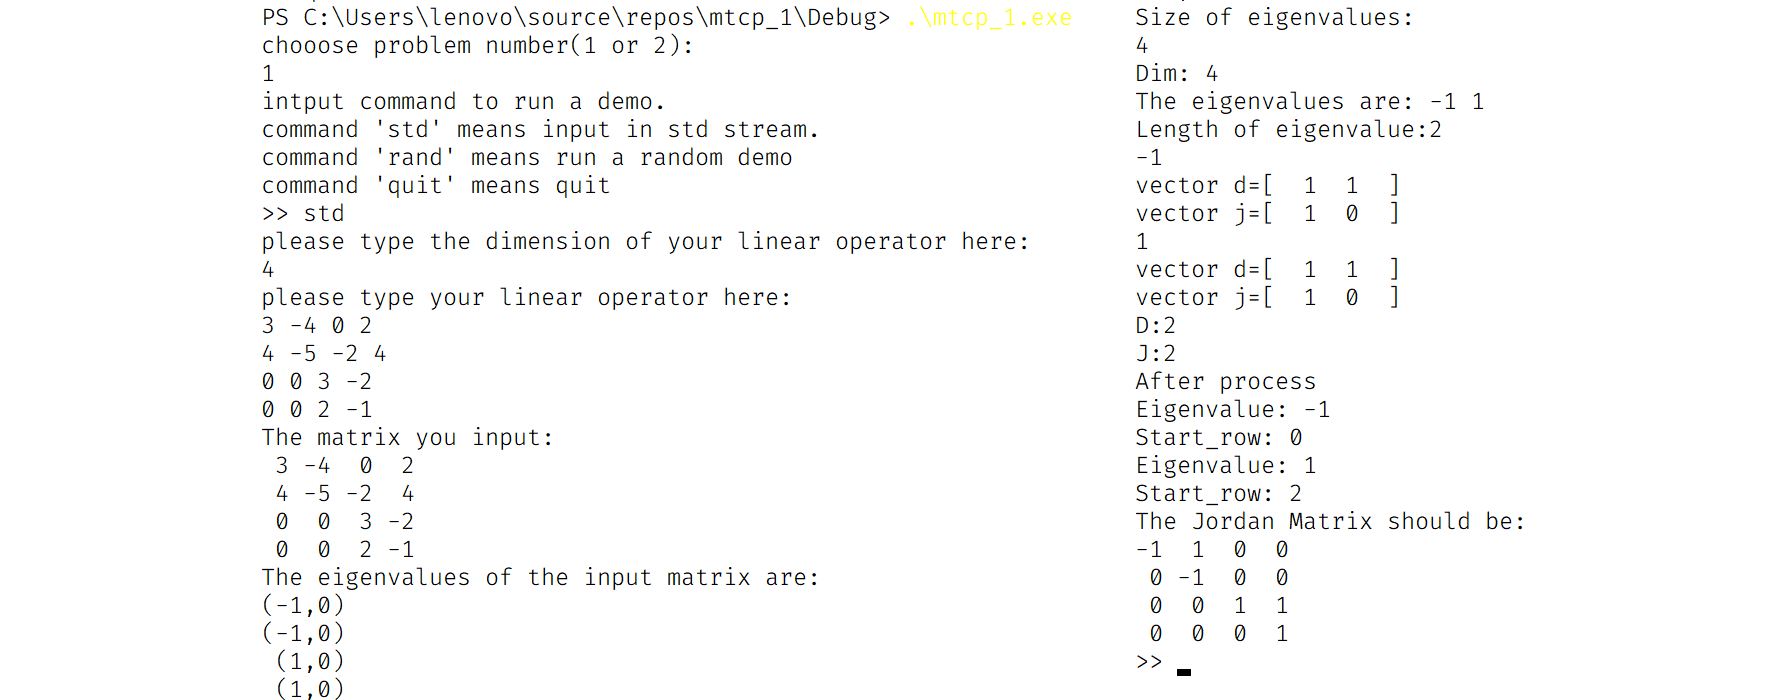
\includegraphics[height = 0.65\textheight]{img/result1.png}
            \caption{demo: input from user-defined matrix}
        \end{figure}
    \end{frame}